\section{Evaluation}
\label{sec:eval}

We have implemented our approach in \toolname: a system for repairing parse
errors for \python at its entirety. Next, we describe our implementation and an
evaluation that addresses four questions:

\begin{itemize}
    \item \textbf{RQ1}: How \emph{accurate} are \toolname's predicted error production rules?
                        (\S~\ref{sec:eval:accuracy})
    \item \textbf{RQ2}: How \emph{precisely} can \toolname repair parse errors?
                        (\S~\ref{sec:eval:precise})
    \item \textbf{RQ3}: How \emph{efficiently} can \toolname repair parse errors?
                        (\S~\ref{sec:eval:efficiency})
    \item \textbf{RQ4}: How \emph{useful} are \toolname's suggested repairs?
                        (\S~\ref{sec:eval:useful})
\end{itemize}

% \subsection{Implementation} \label{sec:eval:gen_method}

\mypara{Training Dataset}
For our evaluation, we use the \python dataset we used in our error data
analysis in \autoref{sec:error-analysis} gathered from
PythonTutor.com~\citep{Guo2013} between the years 2017 and 2018. The dataset has
more than 1,100,000 usable erroneous Python programs and their respective fixes.
The programs have an average length of \emph{87 tokens}, while the abstracted
token sequences have a much shorter average of \emph{43 tokens}. We choose
15,000 random programs from the dataset for all our tests, and the rest we use
as our training set.

We first learn a PCFG on the training set of fixed programs to learn
the probabilities for each production rule in the \emph{full \python
grammar}. \toolname then extracts the abstracted token sequences for all
programs in the training set. Next, while the full \python grammar has
\emph{455 possible terminal error production rules}, in reality only \emph{340 error rules} are ever used in our dataset.
We arrive at this set of error rules by parsing all the erroneous programs in
the training set with the ECE-Parser and the "diff" error rules, as described in
\autoref{sec:overview:train}. Each program is assigned as labels these
error rules that make the ECE-Parser parse the erroneous program successfully.

\mypara{Transformer Classifier}
\toolname's error rule prediction uses a Transformer classifier with \emph{six}
transformer blocks, that each has a fully-connected hidden layer of 256 neurons
and 12 attention heads. The output of the transformer blocks is then connected
to a \dnn based classifier with \emph{two} fully-connected hidden layers of 256
and 128 neurons respectively. The neurons use rectified linear units (ReLU) as
their activation function \citep{Nair2010-xg}, while the output layer uses the
sigmoid function for each class \citep{Nielsen2015-pu}. Additionally, the are
\emph{two input embedding layers} of a length of 128, one for input tokens and
one for their positions in the sequence. We also limit the input
abstracted token sequences to a length of 128, which covers $95.7\%$ of the
training set, without the need of pruning them. Finally, the Transformer
classifier was trained using an \textsc{Adam} optimizer \citep{Kingma2014-ng}, a
variant of stochastic gradient descent that converges faster, for a total of 50
epochs.

\subsection{RQ1: Accuracy}
\label{sec:eval:accuracy}

% colors from http://colorbrewer2.org/?type=sequential&scheme=Blues&n=3
\definecolor{blue1}{HTML}{DEEBF7}
\definecolor{blue2}{HTML}{9ECAE1}
\definecolor{blue3}{HTML}{3182BD}
\definecolor{green1}{HTML}{E5F5E0}
\definecolor{green2}{HTML}{A1D99B}
\definecolor{green3}{HTML}{31A354}

\begin{figure}[t]
  % \begin{minipage}[c]{0.49\linewidth}
    \centering
    \resizebox{0.6\linewidth}{!}{
      \Large
      \begin{tikzpicture}
      \begin{axis}[
        ybar stacked,
        width=1.1\linewidth,
        height=11cm,
        % title={Accuracy of Repair Template Prediction},
        ylabel={Prediction Accuracy (\%)},
        bar width=1cm,
        ymin=0.0,
        ymax=101.0,
        ytick={0.0, 10.0, 20.0, 30.0, 40.0, 50.0, 60.0, 70.0, 80.0, 90.0, 100.0},
        yticklabel={\pgfmathparse{\tick}\pgfmathprintnumber{\pgfmathresult}},
        ytick style={draw=none},
        ymajorgrids = true,
        symbolic x coords={original, abstracted, abstracted-best},
        enlarge x limits=0.3,
        xtick=data,
        xtick style={draw=none},
        xticklabels={\textsc{Original}\xspace, \textsc{Abstracted}\xspace, \textsc{Threshold}\xspace},
        %x tick label style={rotate=45, anchor=north east},
        % x tick label style={font=\small},
        % y tick label style={font=\small},
        reverse legend,
        % transpose legend,
        legend style={legend pos = north east, legend columns=4, font=\small},
      ]

      \addplot[draw=black, fill=blue2, bar shift=-.501cm, postaction= { pattern=dots }] coordinates {(original, 0.0) (abstracted, 0.0) (abstracted-best, 79.28025102961365)};

      \resetstackedplots

      \addplot[draw=black, fill=green2, bar shift=.501cm, postaction= { pattern=dots }] coordinates {(original, 0.0) (abstracted, 0.0) (abstracted-best, 69.82968369829683)};

      \resetstackedplots

      \addplot[draw=black, fill=green1, bar shift=.501cm] coordinates {(original, 12.875536480686696) (abstracted, 58.394160583941606) (abstracted-best, 0.0)};
      \addlegendentry{Top-10}
      \addplot[draw=black, fill=green2, bar shift=.501cm] coordinates {(original, 20.100143061516448) (abstracted, 14.922952149229523) (abstracted-best, 0.0)};
      \addlegendentry{Top-20}
      \addplot[draw=black, fill=green3, bar shift=.501cm] coordinates {(original, 31.974248927038623) (abstracted, 15.49067315490673) (abstracted-best, 0.0)};
      \addlegendentry{Top-50}
      \addlegendimage{empty legend}
      \addlegendentry{Rare:}

      \resetstackedplots

      \addplot[draw=black, fill=blue1, bar shift=-.501cm] coordinates {(original, 56.712132089016514) (abstracted, 72.11217885859972) (abstracted-best, 0.0)};
      \addlegendentry{Top-10}
      \addplot[draw=black, fill=blue2, bar shift=-.501cm] coordinates {(original, 11.769733018835673) (abstracted, 9.335163757599531) (abstracted-best, 0.0)};
      \addlegendentry{Top-20}
      \addplot[draw=black, fill=blue3, bar shift=-.501cm] coordinates {(original, 18.65107852186101) (abstracted, 11.253840622344256) (abstracted-best, 0.0)};
      \addlegendentry{Top-50}
      \addlegendimage{empty legend}
      \addlegendentry{All:}

      \end{axis}
      \end{tikzpicture}
    }
    \caption{
      Results of our error production rule prediction classifiers for the simple original token sequences and their abstracted versions using the PCFG.
    }
    \label{fig:accuracy-results}
  % \end{minipage}
  % \begin{minipage}[c]{0.49\linewidth}
  %   \centering
  %   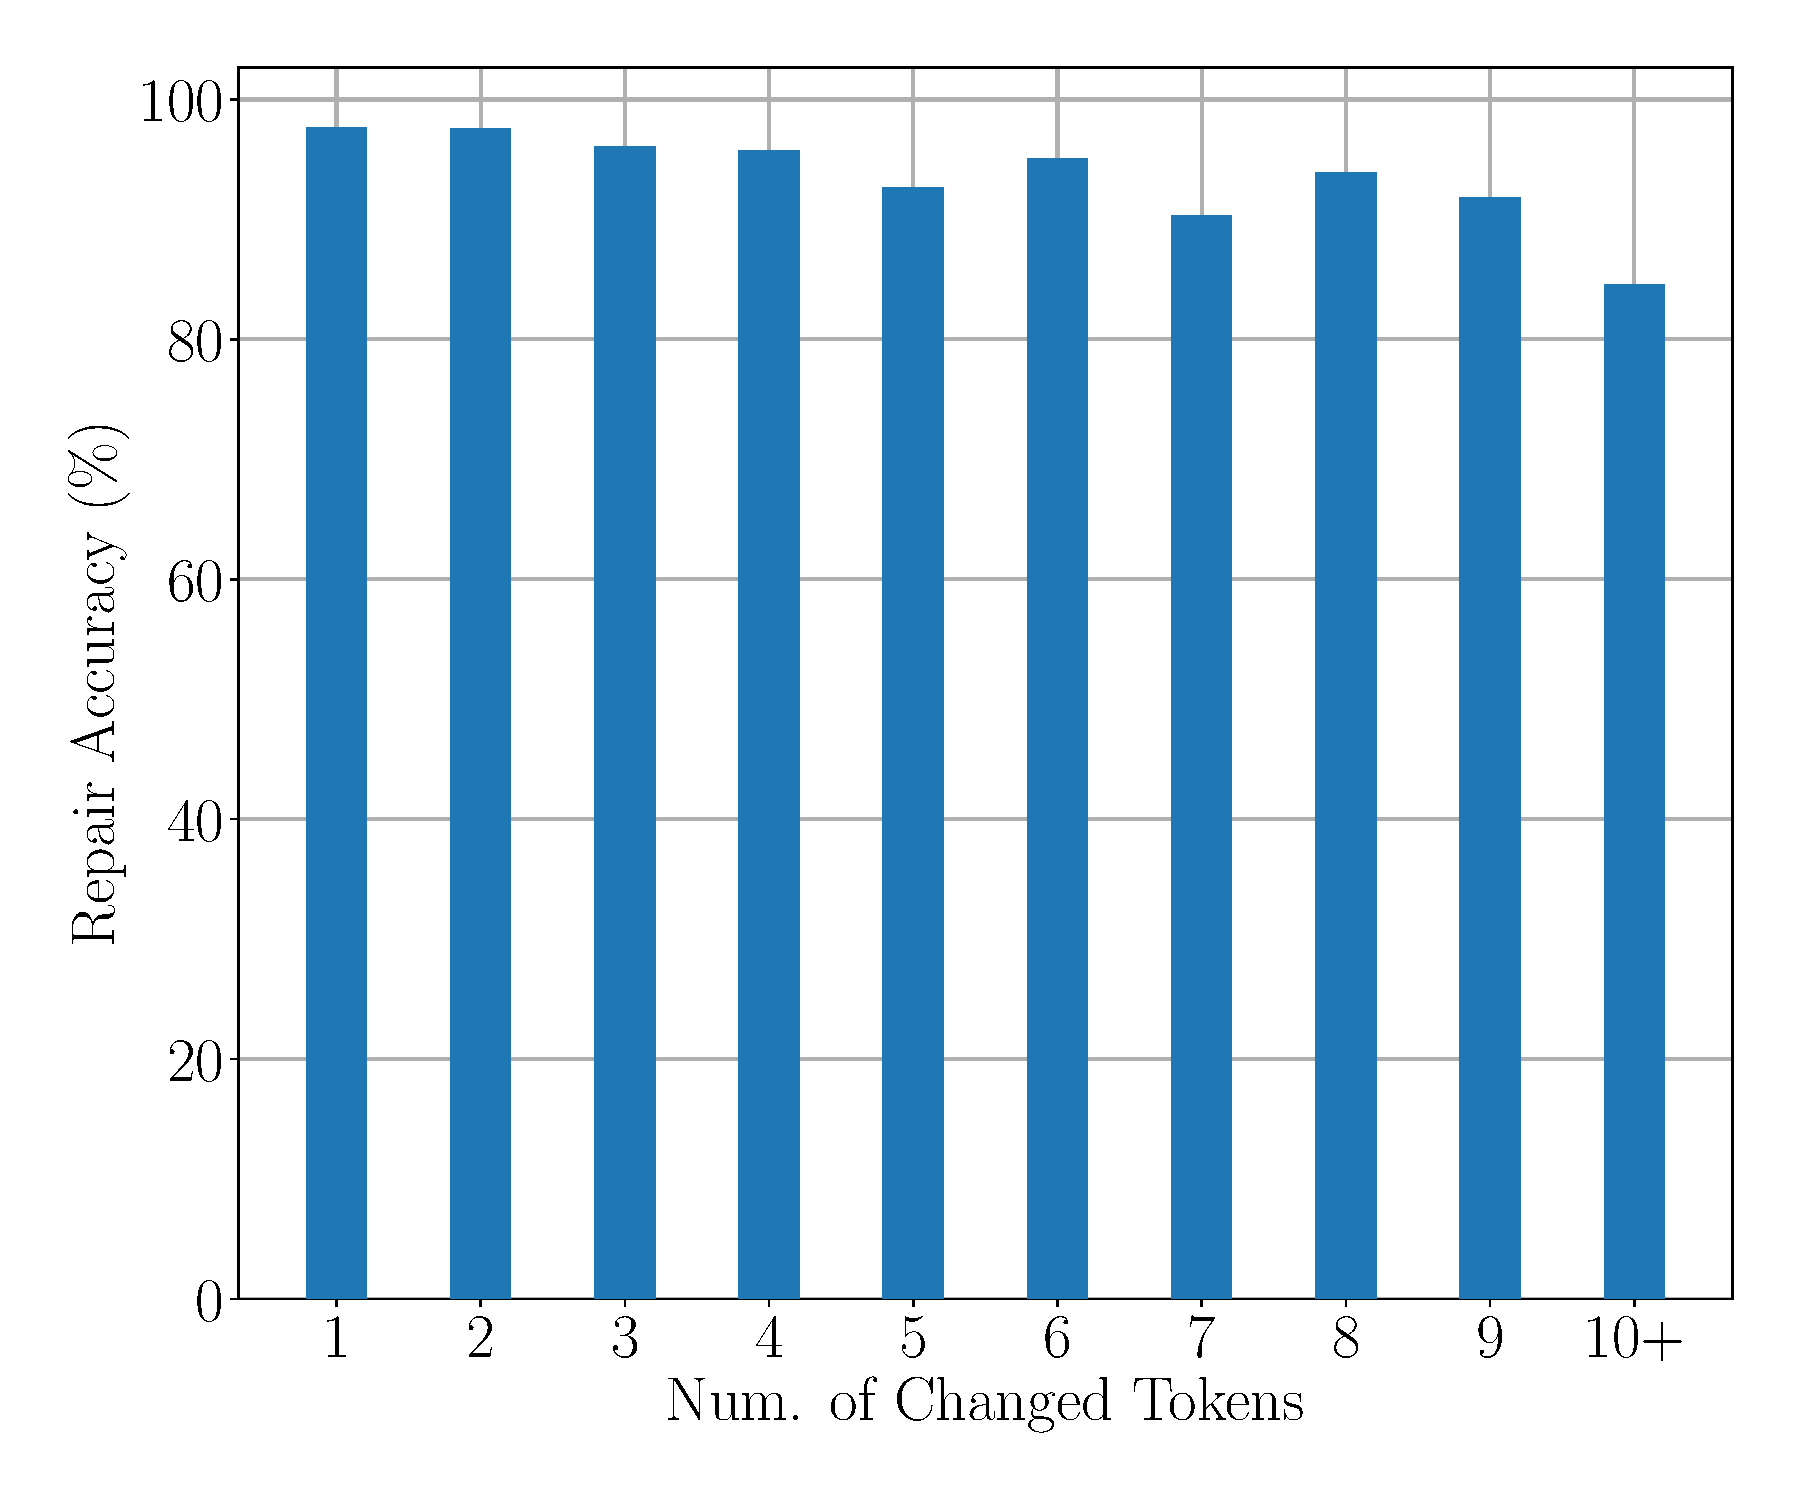
\includegraphics[width=\linewidth]{accuracy-per-change.pdf}
  %   \caption{The repair accuracy for the number of edits needed by the user to repair.}
  %   \label{fig:accuracies-per-changes}
  % \end{minipage}
\end{figure}


% \mypara{Results: Accuracy of Error Rule Prediction}
%
\autoref{fig:accuracy-results} shows the accuracy results of our error
production rule prediction experiments. The y-axis describes the
\emph{prediction accuracy}, \ie the fraction of test programs for which the
correct \emph{full set} of error rules to repair the program was predicted in
the top-K sorted rules.
%
The \textsc{Original} version of our transformer classifier does not consider
the abstracted token sequences and used the full \textsc{Original} token
sequences, whose results are presented in the first two bars of
\autoref{fig:accuracy-results}. The next two bars show our final results using
the \textsc{Abstracted} token sequences to train the classifier. Finally, the
last two dotted bars show the results for when a \textsc{Threshold} is set in
order to select the predicted error rules, instead of picking the static top-K
ones. The predicted error rule set can have a size anywhere between 1 and a
maximum of 25 (pre-defined by us based on the top-K results).

The blue bars show the accuracy on the full test set of \textsc{All} 15,000 test
programs, while the green bars show the results on the subset of the
\textsc{Rare} programs, \ie the programs that did not include any of the 50 most
popular error rules, that amount only for 4.8\% of our test set.

The \textsc{Original} predictor, even with the Top-50 predicted error rules is
less accurate than the Top-20 predictions of the \textsc{Abstracted}, with an
accuracy of 87.13\%, which drops to 68.48\% and 56.71\% respectively for the
Top-20 and Top-10 predictions. The \textsc{Abstracted} predictor significantly
outperforms the \textsc{Original} predictor with a 72.11\% Top-10 accuracy,
81.45\% Top-20 accuracy and 92.70\% Top-50 accuracy.

The \textsc{Threshold} predictions are almost as accurate as the
\textsc{Abstracted} Top-20 predictions with an accuracy of 79.28\% and a median
number of selected error rules of 14 (average 14.1). This could potentially mean
that this predictor is a valid alternative for the static Top-20 predictions.

Finally, we observe that our \textsc{Abstracted} classifiers generalize
efficiently for our dataset of erroneous \python programs and is almost as
accurate for the \textsc{Rare} programs as the rest of the dataset with a
73.32\% Top-20 accuracy (88.81\% Top-50 accuracy). The same holds for the
\textsc{Threshold} predictions with a 69.83\% accuracy.

\begin{framed}
  \noindent \toolname's transformer classifier learns to encode programs with
  syntax errors and select candidate error production rules for them
  effectively, yielding \emph{high accuracies}. By abstracting the tokens
  sequences, \toolname is able to \emph{generalize} better and make more
  accurate predictions with a \emph{81.45\% Top-20 accuracy}.
\end{framed}


\subsection{RQ2: Repaired Program Preciseness}
\label{sec:eval:precise}

Next we evaluate \toolname's end-to-end accuracy and preciseness in generating
valid parses for programs with syntax errors. For all of our tests we limit
\toolname's parsing time to \emph{5 mins} and run our experiments on the 15,000
program  test set. Additionally, we use here the highest-performing transformer
classifier, the \textsc{Abstracted} classifier.

We compare \emph{two versions} of our \toolname implementation
(\textsc{AllParses} and \textsc{MinimumCost}) against two versions of the
error-correcting parser with a static selection of the 20 and 50 most popular
error production rules in our training set. We do this because we
observe in our training set that the 50 most popular error rules are used for
parsing as much as \emph{86\%} of the dataset.

Our \textsc{AllParses} ECE-Parser and \textsc{MinimumCost} ECE-Parser both use
the \emph{Top-20 predictions} from our \textsc{Abstracted} classifier to parse
and repair buggy programs. The \textsc{AllParses} ECE-Parser keeps internally
\emph{all possible states} that arise from using the predicted error rules
similarly to the original ECE-Parser described in \citep{Aho_1972}. We use a
maximum repair cost of 2 edits (\ie a maximum of 2 insertions, deletions or
replacements) to limit the search space. The \textsc{MinimumCost} version
however keeps always the minimum-edit repair and discards all other states that
may lead to a higher cost. This allows for a higher maximum cost of 10 edits.
Finally, while \textsc{AllParses} can generate a large number of repairs, we
keep only the top 3 repairs after filtering with a static code checker
(\textsc{Pylint}, \url{https://www.pylint.org/}) as most developers will
consider at most five suggestions before falling back to manual debugging
\citep{Kochhar2016-oc, Parnin2011-ce}.

\autoref{tab:seq2parse_full_results} shows the percentage of test programs that
each of these four versions can parse successfully (\ie the parse accuracy), the
rare programs parse accuracy, and the amount of parses that match the one that
user compiled. We observe that the Top-20 predictions with the
\textsc{MinimumCost} ECE-Parser \emph{outperforms} every other option with
94.25\% parse accuracy and 94.01\% rare parse accuracy. It also
generates the intended user parse for 20.55\% of the set, \ie over 1 out 5 of the
cases. The 20 most popular ECE-Parser with 79.87\% parse accuracy and 65.01\%
rare parse accuracy is much less accurate, and is 4.24\% less likely to
generate the user parse, while the 50 most popular is slightly less accurate
with 91.91\% and 82.70\% accuracy, as expected from the usage of a large number
of popular error rules. The 50 most popular ECE-Parser has also a high user fix
accuracy of 18.61\%. The \textsc{AllParses} ECE-Parser has a lower parse
accuracy of 61.82\%, however it manages to generate the user fix
33.92\% of the time and achieve a high 72.22\% rare accuracy. 
%It thus achieves to
%parse one out of three programs with syntax errors, while also being effective
%to parse even the rare programs. recommends removing due to space

\begin{framed}
  \noindent \toolname can \emph{parse and repair 94.25\%} of programs with
  syntax errors, while also generating \emph{the user fix over 1 out 5 of
  cases}.
\end{framed}

% \begin{table}[t]
%   \centering
%   \begin{tabular}{l||cccc}
%     Error Rule Approach            & Parse Accuracy & User Parse Rate & Parse time & Speedup \\
%     \hline
%     20 Most Popular                & 79.81\% & 16.31\% & 4.8 sec  & 45.8 sec \\
%     50 Most Popular                & 90.03\% & 18.55\% & 10.6 sec & 37.1 sec \\
%     Top-20 (\textsc{AllParses})   & 59.31\% & 30.57\% & 15.6 sec & 57.4 sec \\
%     Top-20 (\textsc{MinimumCost}) & 92.45\% & 19.95\% & 5.3 sec  & 68.0 sec \\
%   \end{tabular}
%   \caption{Experimental results of \toolname's repair approaches.}
%   \label{tab:seq2parse_full_results}
% \end{table}

\begin{figure}[t]
  \centering
  \begin{minipage}[c]{0.46\linewidth}
    \centering
    \resizebox{\linewidth}{!}{
      \begin{tabular}{l||ccc}
        Error Rule            & Parse            & Rare Parse       & User Fix \\
        Approach              & Accuracy         & Accuracy         & Accuracy \\
        \hline
        20 Most Popular       & 79.87\%          & 65.01\%          & 16.31\% \\
        50 Most Popular       & 91.91\%          & 82.70\%          & 18.61\% \\
        \textsc{AllParses}    & 61.82\%          & 72.22\%          & \textbf{33.92\%} \\
        \textsc{MinimumCost}  & \textbf{94.25\%} & \textbf{94.01\%} & 20.55\% \\
      \end{tabular}
    }
    \caption{Experimental results of \toolname's repair approaches.}
    \label{tab:seq2parse_full_results}
  \end{minipage}
  \begin{minipage}[c]{0.53\linewidth}
    \centering
    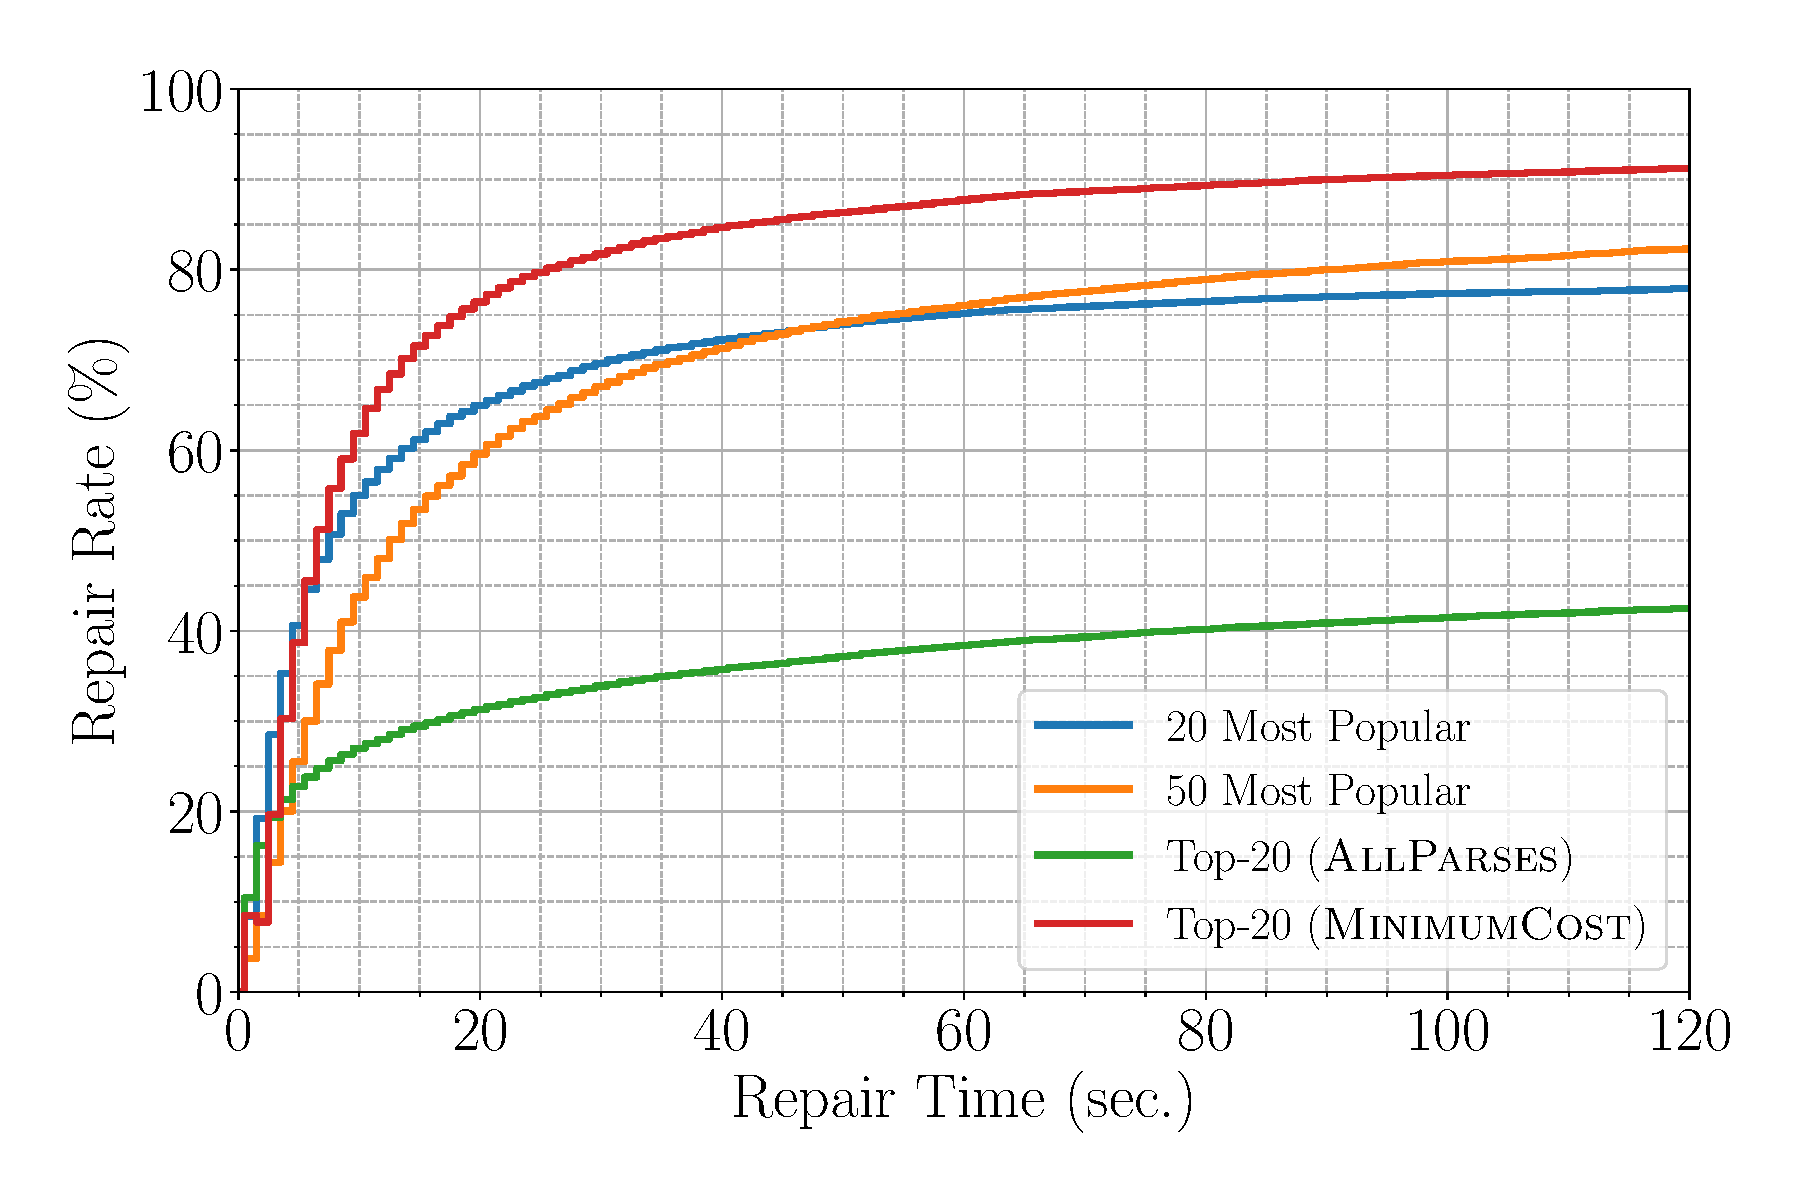
\includegraphics[width=\linewidth]{tool-repair-rate.pdf}
    \caption{The repair rate for all the approaches in
    \autoref{tab:seq2parse_full_results}}
    \label{fig:tool-repair-rate}
  \end{minipage}
\end{figure}

\subsection{RQ3: Efficiency}
\label{sec:eval:efficiency}

% \begin{figure}[t]
%   \centering
%   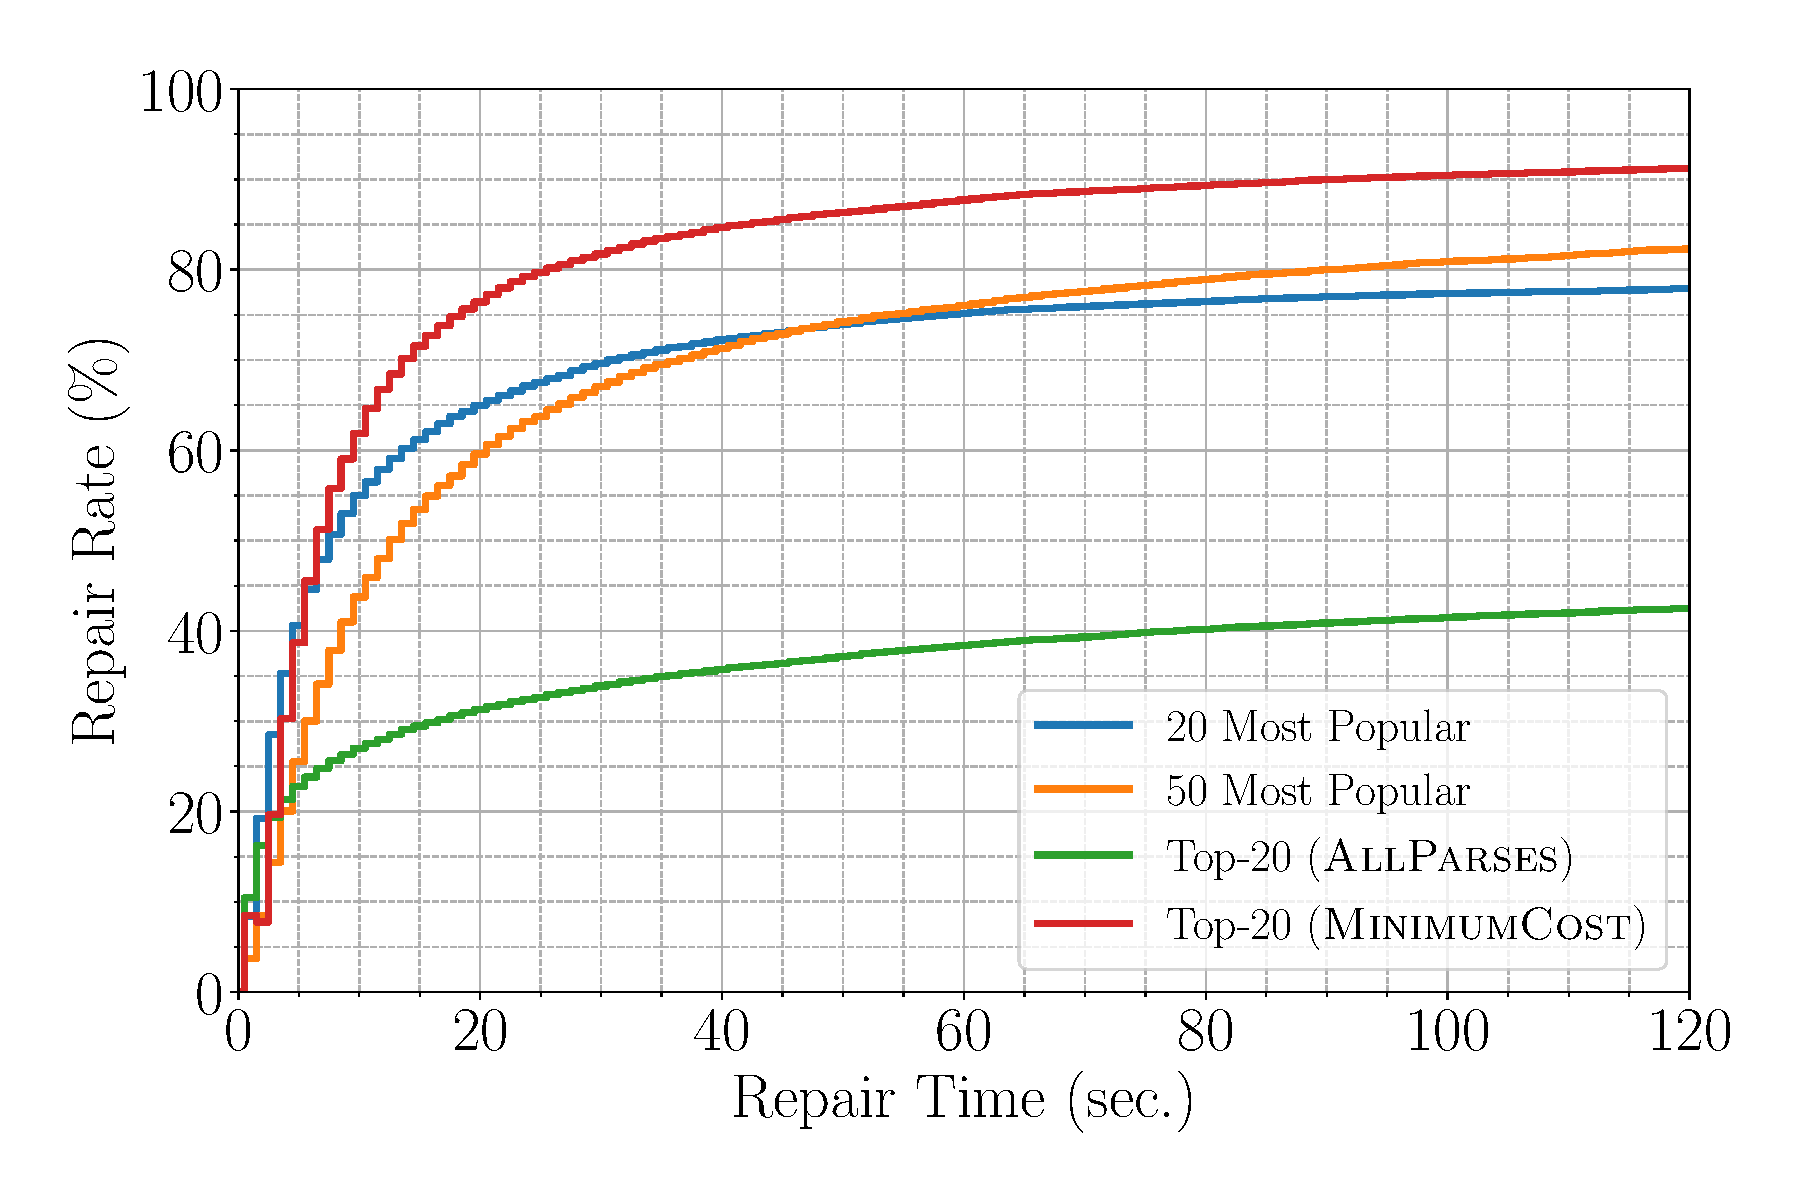
\includegraphics[width=0.8\linewidth]{tool-repair-rate.pdf}
%   \caption{The repair rate for all the approaches in
%   \autoref{tab:seq2parse_full_results}}
%   \label{fig:tool-repair-rate}
% \end{figure}

Next we evaluate \toolname's efficiency by measuring how many programs it is
able to parse. We limit each ECE-Parser to 5 minutes. (In general the procedure
is undecidable, and we conjecture that a longer timeout will diminish the
practical usability for novices.) We compare the efficiency of \toolname for all
the versions of \autoref{tab:seq2parse_full_results}.

\autoref{fig:tool-repair-rate} shows the cumulative distribution function of all
\toolname approaches' repair rates over their parse time. We observe that using
the top 20 error production rule predictions is the most efficient while
maintaining the highest parse accuracy at all times, with a repair rate of
78.10\% within 20 seconds and a median parse time of 5.3 seconds.

We observe that, using a fixed set of the 20 and 50 most popular rules for
\toolname to parse programs with syntax errors, a 61.41\% and 65.20\%
respectively within 20 seconds, and median parse times of 7.0 and 10.1 seconds
respectively. The 50 most popular ECE-Parser is parses less programs until the
45 seconds but the extra number of error rules aids the ECE-Parser to parse more
after that point and outperform the 20 most popular ECE-Parser.

We also observe that \toolname successfully parses around 38.50\% of the
programs with its \textsc{AllParses} approach in 20 seconds and has a median
parse time of 23.2 seconds. While this approach is much less efficient that the
others. due to the vast amount of states is keeps internally in its data
structure, it is also able to generate the exact human repair in 1 out of 3
times which makes still a very valuable approach (\S~\ref{sec:eval:precise}).

\begin{framed}
  \noindent \toolname can parse programs with syntax errors for the vast
  majority of the test set in under 20 seconds.
\end{framed}

\subsection{RQ4: Usefulness}
\label{sec:eval:useful}

% FIXME - define word for non-equivelent repairs

As \toolname's is intended as an aid for programmers
faced with parse errors, we are also interested in the subjective 
human understanding of the quality
and helpfulness of our repairs. 31\% of repairs produced by \toolname
using its \textsc{AllParses} approach are identical to the historical human repair
and thus likely helpful for programmers. However, it may be that \toolname's fixes
are still helpful for debugging even when they differ from the human
repair (\ie \textit{non-equivelent} repairs). To investigate this hypothesis, 
we conduct a human study of the quality and debugging helpfulness of \toolname non-equivalent fixes.

\mypara{Human Study Setup.} We recruited participants from two large public
research institutions (names omitted for blind-review) and through Twitter.
The study was online, took around 30 minutes, and participants could enter a
drawing for one of two \$50 awards. In the study, participants
were each asked to rate 15 debugging hints randomly selected from a corpus of 50
stimuli\footnote{All human study stimuli are included in our replication
package at {link removed for blind review}}.

We created the stimuli by selecting 50 buggy programs from the Python Tutor dataset
for which \toolname and the historical human produced different fixes. Other than
ensuring a wide array of difficulty (as assessed by how long the
human took to fix the error), programs were selected randomly. Each 
stimulus consisted of a buggy program, its associated syntax 
error message, and a potential program fix presented as a \emph{debugging hint}. 
For each stimulus, we produced two versions: one where the debugging hint was 
generated by \toolname and one where the debugging hint was the historical 
human-created fix. 
Participants rated the quality and helpfulness of each debugging
hint using a 1-5 Likert scale.
They also indicated if the debugging hint provided helpful information beyond
that in the Python error message %\footnote{In this study, we used error messages from Python 3.10. Compared to earlier Python versions, 3.10 includes improved error messages for Syntax Errors.}.
Participants were unaware of if any given
hint was generated by a human or \toolname, and participants were never shown both the
tool-generated and human-generated repairs to the same buggy program. To be included
in analysis, participants had to assess at
least four stimuli. Overall, we analyze 527 unique stimuli ratings from 39 valid
participants (246 for human-generated foxes and 281 for \toolname fixes).

\mypara{Overall Results.} While humans in our study find that non-equivelent repairs produced by
\toolname are lower in both quality and debugging helpfulness than those produced 
by humans (2.9/5 helpfulness for tool-produced repairs vs 3.7/5 for human-produced 
repairs, $p < 0.001$), humans still often find \toolname's fixes 
helpful for debugging: participants found that \toolname repairs contained helpful 
debugging information beyond that contained in the Python Error message 48\% of 
the time (134/281). This additional helpful debugging information was often in both
the content (73\% of the time) and location (55\% of the time) of the generated
repair. Additionally, \toolname fixes are helpful for easy and hard Syntax Errors
alike: we found no statistically significant difference between the helpfulness or
quality of \toolname's repairs for easy parse errors (those repaired by the human in under
40 seconds) or hard parse errors (those repaired by the human in over 40 seconds). %p = 0.07 and 0.13 respectively if we have room to include
Overall, these results indicate that even when \toolname repairs differ from
that of the historical human repair, they may still often be helpful for debugging.

\mypara{Individual Stimuli.} Beyond an analysis of \toolname's overall quality, we also 
analyze the helpfulness of each stimulus. % FIXME: If room, can add more statistical details if needed
Of the 48 programs for which we collected sufficient data to permit statistical 
comparison, the user repair was statistically more helpful for debugging than \toolname's
repair for 33\% of stimuli (16/48, $p<0.05$). However, we found that \toolname's
repair was actually \emph{more helpful} for debugging than the human's repair for 15\% of
stimuli (7/48, $p<0.05$). For the remaining 52\% of stimuli, we found no evidence of a 
statistical difference in the debugging helpfulness of the two repairs.

\begin{figure}[h]
  \centering
  \begin{minipage}[c]{0.47\linewidth}
  \begin{python2}
# Buggy
def gcdIter(a, b):
    for i in range(1, a+1):
        if a % i == 0:
        elif b % i == 0:
    return i 
gcdIter(9, 12)
  \end{python2}
  \begin{python2}
# Human
def gcdIter(a, b):
    for i in range(1, a+1):
        return a % i
gcdIter(9, 12)
  \end{python2}
  \begin{python2}
# Seq2Parse
def gcdIter(a, b):
    for i in range(1, a+1):
        if a % i == 0: new_var
        elif b % i == 0: break
    return i
gcdIter(9, 12)
  \end{python2}
  \subcaption{\toolname repair significantly more helpful:
  4.3/5 vs 1.0/5, $p = 0.03$}
  \label{fig:proga}
  \end{minipage}%
  \hspace{0.02\linewidth}%
  \begin{minipage}[c]{0.47\linewidth}
    \begin{python2}
aList = [12, 'yz', 'ab'];
aList.reverse();
print "List : ", aList  
    \end{python2}
    \begin{python2}
aList = [12, 'yz', 'ab']
aList.reverse() 
    \end{python2}
    \begin{python2}
aList = [12, 'yz', 'ab']
aList.reverse()
print("List : ", aList)
    \end{python2}
    \subcaption{\toolname repair significantly more helpful:
    4.75/5 vs 2.0/5, $p = 0.02$}
    \label{fig:progb}

    \begin{python2}
a = int(input(enter a))
print(a***3)
    \end{python2}
    \begin{python2}
a = int(input("enter a"))
print(a**3)
    \end{python2}
    \begin{python2}
a = int(input(enter)(a))
print(a ** (* 3))
    \end{python2}
    \subcaption{Historical human repair significantly more helpful:
    1.8/5 vs 4.75/5, $p = 0.01$}
    \label{fig:progc}
    \end{minipage}%
      
  \caption{Three example buggy programs followed by their historical human
  and \toolname repairs. For (a) and (b), \toolname's repair
  was rated more helpful by participants. For (c), the human
  repair was more helpful.}
  \label{fig:user_study_examples}
\end{figure}

To better contextualize these results, we provide examples of stimuli with
statistically significant differences in debugging helpfulness. 
In figure~\ref{fig:progb}, \toolname's repair was 
significantly more helpful than the user repair: 
 \toolname correctly adds parentheses to \texttt{print} 
while the human simply deletes the 
buggy line, perhaps out of confusion or frustration.
Similarly, figure~\ref{fig:proga}'s \toolname repair was also
better than the user repair. In this case, the user appears to try to
implement a function to calculate the greatest common divisor of two integers,
but has empty \texttt{if} and \texttt{elif} statements. 
To ``fix'' this bug, the user
deletes the \texttt{if} and \texttt{elif} and modifies the return statement.
However, this fix does not correctly calculate the greatest common divisor.
\toolname, on the other hand, adds a template variable to the \texttt{if} and 
\texttt{break} to the \texttt{elif}. While this also does not implement
greatest common divisor, it is likely closer to the intended final solution
than the user repair. This example also demonstrates the beneficial ability of our approach
to conduct multi-edit repairs. 

Figure~\ref{fig:progc}, on the other hand, contains an example of when the
human repair was more helpful than \toolname's repair. In this case, the
human correctly deletes the extraneous \texttt{*} in the power operator
while \toolname adds parentheses to make a more complex expression. 
FIXME: add last line here saying why that is.

\begin{framed}
  \noindent 
Even when non-equivalent to the user's fix, \toolname's repairs are still useful and helpful:
they contain debugging information beyond that in the Python error message 48\% of the time. 
Additionally, two-thirds of \toolname's fixes were either indistinguishable from
or better than those produced by humans for helping debugging.
\end{framed}
